\documentclass[jou, apacite]{apa6}
\usepackage{threeparttable}
\usepackage{amsmath}
\usepackage{amsfonts}
\usepackage{amssymb}
\usepackage{bm}
\usepackage{graphicx}
\graphicspath{ {./Images/} }

\raggedbottom

\begin{document}
\title{Evaluating Main Effects in the Generalized Linear Model}
\shorttitle{Interpreting GLM Main Effects}

\fiveauthors{Max A. Halvorson}{Xiaolin Cao}{Connor J. McCabe}{Dale S. Kim}{Kevin M. King}
\fiveaffiliations{University of Washington}{University of Washington}{University of Washington}{University of California, Los Angeles}{University of Washington}

\abstract{}

\keywords{count models, logistic regression, generalized linear models, data visualization}

\rightheader{Evaluating GLM Main Effects}
\leftheader{Halvorson, Cao, McCabe, Kim, and King}

\maketitle

\section{Introduction}
The odds of having drank any alcohol during the past weekend are 1.8 times higher (p < .001) amongst those who act rashly when experiencing positive emotion (i.e., low on positive urgency), controlling for the effect of gender.

What is the probability of drinking alcohol on a given day for a person who is low on positive urgency? How about for someone who is high on positive urgency? Is this effect stronger for men? Stronger for women? Or equivalent across men and women?

If these questions are difficult to answer, it's not because you've forgotten what you learned in the first couple years of graduate school - it's because this problem is unsolvable, given the information above. 

Recent work has called for more widespread use of extensions of the general linear model which fit implicit assumptions about the data generation process. 
To facilitate this work, tutorials, software examples, and widely-available software packages make fitting these models more and more accessible (Atkins et al., 2007; Atkins \& Gallop, 2013).

Despite widespread use of count and binary outcome models, very few (lit search results) researchers report model results in terms of the quantities of interest (QOI) they set out to understand. 
We found only two manuscripts out of 55 using binary or count outcomes in the Journal of Abnormal Psychology and Journal of Consulting and Clinical Psychology between 2007 and 2017 that followed these recommendations. (FOOTNOTE) 
Literature search was conducted using the same criteria as Norton (2004) and/or Brambor, Clark, \& Golder (2006). 

To make results easier to understand, methodologists recommend that GzLM parameters are best represented 1) in units that are most substantively meaningful and 2) at specific covariate values of interest.
In count models, this entails reporting predicted counts, and in binary outcome models, this entails reporting predicted probabilities of an event occurring. 
We advocate for presenting quantities of interest directly, as fitted models are readily able to output direct predictions of these quantities. 
Thoughtful graphical and tabular presentation of data can facilitate intuition even when models are complicated, and present a richer source of information than single parameters. 

\section{Interpretation of Single Coefficients does not Characterize Generalized Linear Models}
In examining predicted counts and probabilities, it becomes apparent that the single parameters reported in GzLMs do not map onto relationships between predictors and outcomes as readily as they do in ordinary least squares (OLS) regression. 
In fact, further analysis of these parameters reveals that even their transformed versions, such as odds ratios and rate ratios, a) do not represent constant first differences in QOI, and b) do not describe effects that are conditionally independent from one another, as in OLS regression. 
To demonstrate that these two properties hold for binary outcome and count models, we present a simulated-data example with two predictors for each model below. 


\section{The Generalized Linear Model}
%Stolen directly from Dale's paper for now
Generalized linear models are those for which a link function is used to describe the relationship between predictors and the outcome they predict, when the relationship is not well described by a straigh tline. 
The mathematical formulation for any GLM can be shown as:

\begin{equation}
g(\mathbb{E}[Y|\bm{X}]) = \bm{X} \beta ,
\end{equation}

where $g(\cdot)$ is the link function, $\bm{X}\beta$ are linear predictors, and $\mathbb{E}[Y|\bm{X}]$ is taken with respect to the probability distribution. In essence, the link function $g(\cdot)$ transforms the left side of the equation so that the relation between Y and X is not simply a direct relationship with slope $\beta$; rather, the entire left side of the equation varies with $\bm{X}\beta$.
Herein lies some of the ambiguity associated with results of GzLMs.
In this form, we lose sight of the idea that our QOI is the argument to the link function rather than the entire left side of the equation.

In the case of linear reression, there is an implicit identity function serving as the link function.
However, this link function can take many forms, all of which imply a particular data generative process underlying the data themselves.
Link functions take the shape of a relationship between a predictor and an outcome (in linear regression, the slope of a line) and allow that relationship to take on whatever shape is defined by the link function.

The link function we choose embodies our assumptions about the process that generates our data.
In the case of OLS regression, we assume that our outcome is generated by a process with normally distributed errors.
In the case of logistic regression, we assume that there is a latent variable representing underlying levels of some trait. 
For example, a person's diagnostic status as depressed or non-depressed represents an underlying level of continuous depression. 
Using a logit function, we can translate this latent level into a predicted probability of an outcome occurring.
The link function allows predictor variables to influence this latent variable continuously, and describe the effect in terms of changes in probability of occurrence.
\section{Binary Outcome Models}

Binary outcome models involve predicting the probability of an outcome occurring (vs. not occurring) based on a set of predictors. 
The QOI researchers tend to be most interested in is the predicted probability of an occurrence (e.g., of a disease) for individuals with a characteristic or set of characteristics.
More specificallly, research questions tend to focus on how strongly a change in a predictor affects the probability of an outcome occurring.
Motivated by parsimony and led by software defaults, scientists typically report effects of predictors in terms of a single odds ratio.
This practice not only leads to coefficients with unintuitive interpretations, but also implies an independence of covariates and a constancy of the reported effect that are inconveniently untrue.

\subsection{The Logistic Model}

The logistic model is formulated as follows:

\begin{equation} \label{log1}
\pi_i = \dfrac{\exp (X \bm{\beta})}{1 + \exp (X \bm{\beta})},
\end{equation}

\begin{figure}[h]
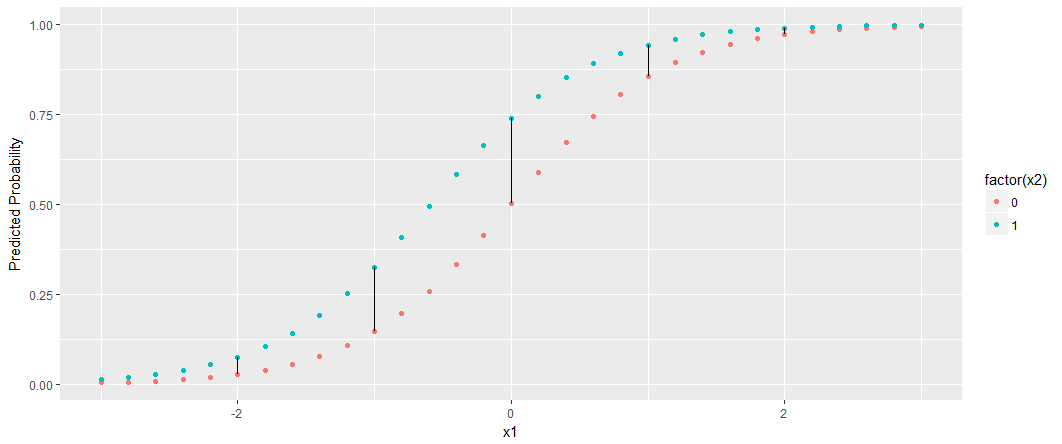
\includegraphics[width=0.5\textwidth]{LogisticFirstDiff.png}
\end{figure}

Since the logit link function is log-linear - that is, it relates to predicted probabilities through a log function - the extent of change in Y for a 1-unit increas in X is not linear. 
An odds ratio describes the relation between the odds of an outcome occurring and the odds of an outcome not occurring, and is a reasonable proxy for the percentage increase in probability, at least when proportions are small.
Unfortunately, an odds ratio provides no information regarding the magnitude of predicted probabilities.

Figure X depicts the relation between a continuous predictor $X_1$, a categorical predictor $X_2$, and the model-predicted probability of a binary outcome Y occurring. 
The curve of each line makes it visually clear that a unit increase in $X_1$ does not lead to a constant increase in $P(Y)$.
Similarly, the black lines between the curves for $X_2=0$ and $X_2=1$ are different lengths, demonstrating visually that the effect of $X_2$ (the amount that the blue line is above the red line) varies based on the level of $X_1$.
Thus, even without interaction terms in a model, effects in logistic regression are not independent from one another. 

\section{Count Models}

\subsection{The Poisson Model}

\begin{equation} \label{pois1}
\mathbb{P}(Y_i = y_i|x_i) = \dfrac{\lambda_i^{y_i}e^{-y_i}}{y_i!}, \quad\text{for } y_i = 0, 1, \dots
\end{equation}
\begin{equation} \label{pois2}
\mathbb{E}[Y_i|x_i] = \lambda_i = \exp (x_i^T \bm{\beta})
\end{equation}

\begin{figure}[h]
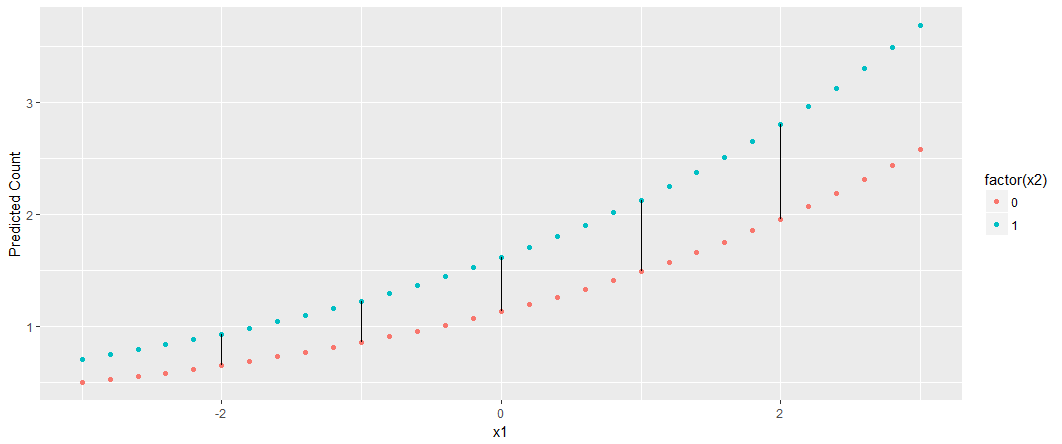
\includegraphics[width=0.5\textwidth]{PoissonFirstDiff.png}
\end{figure}
EXPLAIN INCIDENT RATE RATIOS

\subsection{The Negative Binomial Model}

negative binomial formulation:

\begin{equation}
\mathbb{P}(Y_i = y_i | x_i) = \dfrac{\Gamma(y_i + \theta)}{\Gamma(\theta)y_i!}
  \cdot
  \dfrac{\lambda_i^{y_i}\theta^{\theta}}{(\lambda_i + \theta)^{(y_i + \theta)}},
\end{equation}
\begin{equation}
\mathbb{E}[Y_i|x_i] = \lambda_i = \exp (x_i^T \bm{\beta}),
\end{equation}
where $\Gamma(\cdot)$ is the gamma function and $\theta$ is a constant shape parameter.

The negative binomial model is a generalization of the poisson model with an extra parameter, allowing for non-constant exposure. As such, the properties of non-constant first differences and non-independence of regression coefficients apply. 


\subsection{The Hurdle Model}

hurdle model formulation:

\begin{equation}
\mathbb{P}(Y_i = y_i|x_i) =
  \begin{cases}
    \pi_i, & \text{if } y_i = 0 \\
    (1 - \pi_i)\mathbb{P}_c(Y_i = y_i|x_i), & \text{if } y_i = 1, 2, \dots
  \end{cases}
\end{equation}
\begin{equation}
\pi_i = \dfrac{\exp (x_i^T \bm{\beta}_{\pi})}{1 + \exp (x_i^T \bm{\beta}_{\pi})},
\end{equation}
\begin{equation}
\mathbb{E}[Y_i|x_i] = (1 - \pi_i)\mathbb{E}_c[Y_i|x_i], % Placeholder - Verify
\end{equation}
where $\pi_i$ is once again assumed to be a Bernoulli parameter with logit link.

The hurdle model is a piecewise model involving 1) a logistic regression portion which accounts for zeros and 2) a poisson (or other count) model to account for non-zero values. Hurdle models assume a two-step data generating processes: one that explains whether an observation was a 0 or a positive count (portion 1), and one that predicts that positive count (2). As these models are composed of the aforementioned models, the properties of non-constant first differences and non-independence of regression coefficients applies. 

\subsection{The Zero-Inflated Model}

zero-inflated model formulation:
\begin{equation}
\mathbb{P}(Y_i = y_i|x_i) =
  \begin{cases}
    \pi_i + (1 - \pi_i)\mathbb{P}_c(Y_i = 0|x_i), & \text{if } y_i = 0 \\
    (1 - \pi_i) \mathbb{P}_c(Y_i = y_i|x_i), & \text{if } y_i = 1, 2, \dots
  \end{cases}
\end{equation}
\begin{equation}
\pi_i = \dfrac{\exp (x_i^T \bm{\beta}_{\pi})}{1 + \exp (x_i^T \bm{\beta}_{\pi})},
\end{equation}
\begin{equation}
\mathbb{E}[Y_i|x_i] = (1 - \pi_i)\mathbb{E}_c[Y_i|x_i], % Verify this.
\end{equation}
where $\pi_i$ refers to the probability of an excess zero and $\mathbb{E}_c[Y_i|x_i]$ is the expectation with respect to $\mathbb{P}_c(Y_i|x_i)$.

The zero-inflated model is a piecewise mixture model involving the poisson model (or another count model), which accounts for two processes of generating zeros. Structural zeros, represented by the first term in part 1 of the piecewise function, occur when zeros are thought to be the result of a lack of exposure. Sampling zeros, represented by the second term in part 1 of the piecewise function, are zeros that were sampled from the full count distribution. Positive counts are modeled by part 2 of the piecewise function. As such, the properties of non-constant first differences and non-independence of regression coefficients applies. 


\begin{equation} \label{zip1}
\mathbb{P}(Y_i = y_i|x_i) =
  \begin{cases}
    \pi_i + (1 - \pi_i)e^{-y_i}, & \text{if } y_i = 0 \\
    (1 - \pi_i) \dfrac{\lambda_i^{y_i}e^{-y_i}}{y_i!}, & \text{if } y_i = 1, 2, \dots
  \end{cases}
\end{equation}
\begin{equation} \label{zip2}
\pi_i = \dfrac{\exp (x_i^T \bm{\beta}_{\pi})}{1 + \exp (x_i^T \bm{\beta}_{\pi})},
\end{equation}
\begin{equation} \label{zip3}
\lambda_i = \exp (x_i^T \bm{\beta}_{\lambda}),
\end{equation}
\begin{equation} \label{zip4}
\mathbb{E}[Y_i|x_i] = (1 - \pi_i)\lambda_i,
\end{equation}
where $\pi_i$ refers to the probability of an excess zero as before.


\section{}
When presenting results, it is important to recall that the choice of covariate levels chosen as 0 values can influence the interpretation of results to the majority of readers, who likely do not have the available time or information to probe a model fully. 

We propose that research producers should choose their covariate values thoughtfully. 

In order to characterize an effect accurately, researchers may have to probe an effect at multiple covariate levels, even when no interactions are included in the model.

For example, an interpretation of the above example might be written as follows: There was a main effect of positive urgency on negative alcohol consequences (OR = XX, SE = XX, p = XX). For a 21-year-old male, the predicted number of negative alcohol consequences was 3 for someone low in positive urgencty and 8 for someone high on positive urgency. In contrast, for a 21-year-old female, the predicted number of consequences for 5 for a low-urgency individual and 12 for a high-urgency individual.

Make a comment about cumulative psychological science. This effort is in the direction of quantifying effect sizes, not just reporting p-values. Graphical methods are one means of giving more information about nonlinear models. Another means is to give additional interpretation in the text of results and discussion sections. Especially at the beginning of a discussion section, this type of information can be very useful for readers to contextualize findings. This is also helpful in providing more information and intuition about base rates. But it generally contributes 

\section{Recommendations for Model Reporting: Tables and Graphics}
\subsection{Binary Outcome Data}
Table of first differences with covariate values made explicit

Graphic of first differences for some X1 and X2 of interest	

Real data example???

Show graphs from InterActive? With uncertainty.

\subsection{Count Data}
Table of first differences with covariate values made explicit

Graphic of first differences for some X1 and X2 of interest

Real data example???

Show graphs from InterActive? With uncertainty.
\end{document}
